\documentclass{standalone}
\usepackage{tikz}
\usetikzlibrary{positioning, decorations.pathreplacing}

\begin{document}
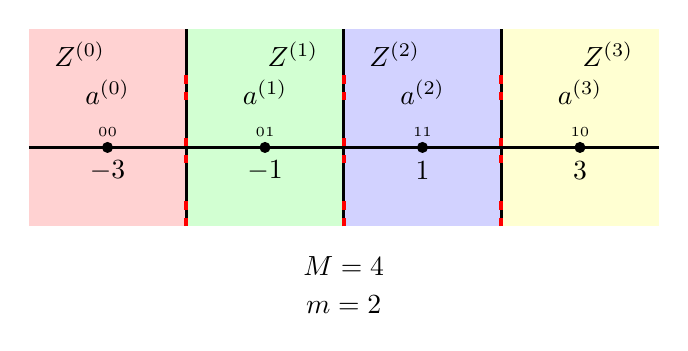
\begin{tikzpicture}

% Define colors
\definecolor{myred}{RGB}{255, 210, 210}
\definecolor{mygreen}{RGB}{210, 255, 210}
\definecolor{myblue}{RGB}{210, 210, 255}
\definecolor{myyellow}{RGB}{255, 255, 210}

% Draw the rectangles
\fill[myred] (-4, 0) rectangle (-2, 2.5);
\fill[mygreen] (-2, 0) rectangle (0, 2.5);
\fill[myblue] (0, 0) rectangle (2, 2.5);
\fill[myyellow] (2, 0) rectangle (4, 2.5);

% Vertical lines in the middle
\draw[very thick] (-2, 0) -- (-2, 2.5);
\draw[very thick] (0, 0) -- (0, 2.5);
\draw[very thick] (2, 0) -- (2, 2.5);

% Draw the dashed lines in red
\draw[red, ultra thick, dashed] (-2, 0) -- (-2, 0.4);
\draw[red, ultra thick, dashed] (-2, 0.8) -- (-2, 1.2);
\draw[red, ultra thick, dashed] (-2, 1.6) -- (-2, 2);

\draw[red, ultra thick, dashed] (0, 0) -- (0, 0.4);
\draw[red, ultra thick, dashed] (0, 0.8) -- (0, 1.2);
\draw[red, ultra thick, dashed] (0, 1.6) -- (0, 2);

\draw[red, ultra thick, dashed] (2, 0) -- (2, 0.4);
\draw[red, ultra thick, dashed] (2, 0.8) -- (2, 1.2);
\draw[red, ultra thick, dashed] (2, 1.6) -- (2, 2);

% Draw the horizontal line
\draw[thick] (-4, 1) -- (4, 1);

% Draw the nodes
\fill (-3, 1) circle (2pt);
\fill (-1, 1) circle (2pt);
\fill (1, 1) circle (2pt);
\fill (3, 1) circle (2pt);

% Add labels
\node at (-3, 1.2) {\textnormal{\tiny $00$}};`'
\node at (-1, 1.2) {\textnormal{\tiny $01$}};
\node at (1, 1.2) {\textnormal{\tiny $11$}};
\node at (3, 1.2) {\textnormal{\tiny $10$}};

\node at (-3, 0.7) {$-3$};
\node at (-1, 0.7) {$-1$};
\node at (1, 0.7) {$1$};
\node at (3, 0.7) {$3$};

\node at (-3, 1.7) {$a^{(0)}$};
\node at (-1, 1.7) {$a^{(1)}$};
\node at (1, 1.7) {$a^{(2)}$};
\node at (3, 1.7) {$a^{(3)}$};

\node[above right] at (-3.8, 1.9) {$Z^{(0)}$};
\node[above left] at (-0.2, 1.9) {$Z^{(1)}$};
\node[above right] at (0.2, 1.9) {$Z^{(2)}$};
\node[above left] at (3.8, 1.9) {$Z^{(3)}$};

% Add the bottom text
\node at (0, -0.5) {$M=4$};
\node at (0, -1) {$m=2$};

\end{tikzpicture}
\end{document}


